\begin{figure*}[!h]
\begin{subfigure}{0.24\linewidth}
\centering
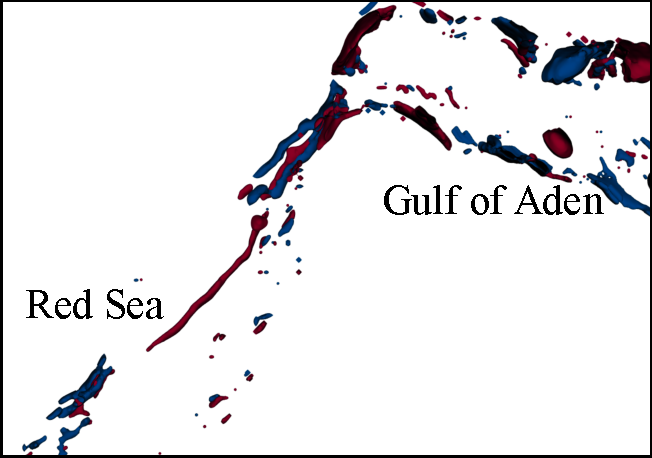
\includegraphics[width=\linewidth]{Images/RedSeaEddy/zls.pdf}
\vspace{-2mm}
\caption{$ZLS_{T}$}
\label{fig:rse_zls}
\end{subfigure}
\begin{subfigure}{0.24\linewidth}
\centering
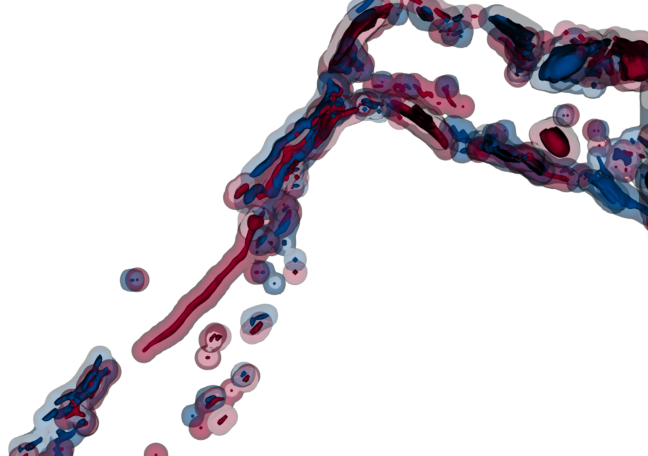
\includegraphics[width=\linewidth]{Images/RedSeaEddy/fls_6.pdf}
\vspace{-2mm}
\caption{$ZLS_{T}$ + $FLS_{T,6}$}
\label{fig:rse_fls}
\end{subfigure}
\begin{subfigure}{0.24\linewidth}
\centering
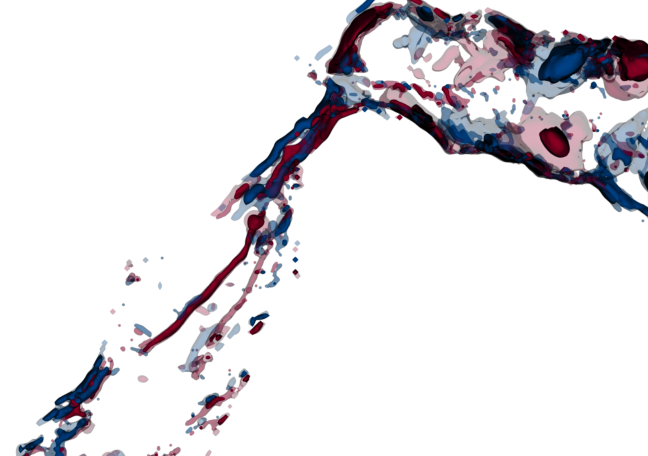
\includegraphics[width=\linewidth]{Images/RedSeaEddy/fcls_68.pdf}
\vspace{-2mm}
\caption{$ZLS_{T}$ + $FCLS_{T,68\%}$}
\label{fig:rse_fcls}
\end{subfigure}
\hfill
\begin{subfigure}{0.24\linewidth}
\centering
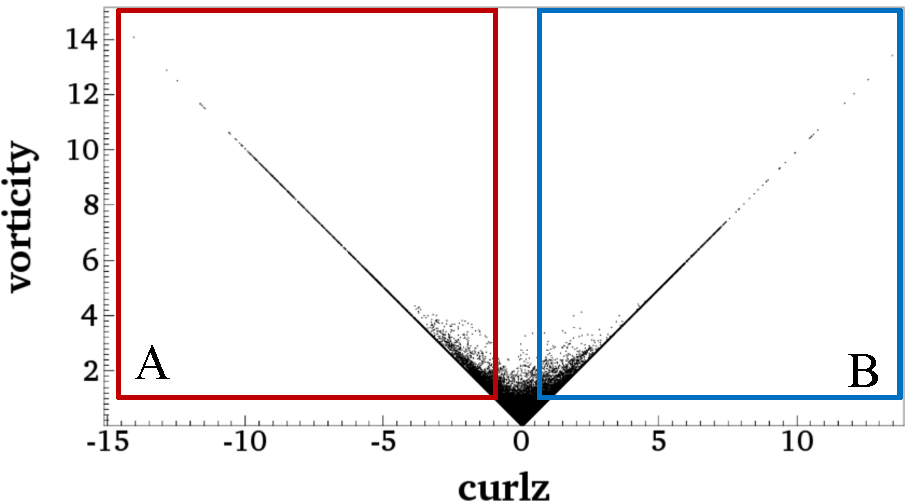
\includegraphics[width=0.95\linewidth]{Images/RedSeaEddy/scatterplot.pdf}
\vspace{-2mm}
\caption{Attribute space 2D scatterplot and, traits (rectangular selections). We use $T = \left\{T_{A}, T_{B}\right\}$.} 
\label{fig:rse_scatterplot}
\end{subfigure}
\vspace{-2mm}
\caption{Visualization of anticyclonic~($T_{A}$, red) and cyclonic~($T_{B}$, blue) eddies in the Gulf of Aden and part of the Red Sea using the derived attributes of vorticity magnitude and the z-component of curl.}
\vspace{-2mm}
\label{fig:rse}
\end{figure*}
